\section{Modularisierung}
Modularisierung ist die Aufteilung eines Ganzen in Teile, die als Module oder Komponenten bezeichnet werden. Bei geeigneter Form und Funktion können sie zusammengefügt werden oder über entsprechende Schnittstellen interagieren.

\subsection{Grundprinzip}
\begin{itemize}
  \item Divide et impera (Teile und herrsche)
  \begin{itemize}
    \item Problem aufteilen und Unterprobleme einzeln angehen
    \item Zuerst Grobentwurf, dann verfeinern (Top-Down-Prinzip)
  \end{itemize}
  \item \textbf{Ziel:} Reduktion der Komplexität
\end{itemize}

\subsection{Motivation}
Bei Kleinstsoftware braucht es kein systematisches Design, da man diese meist auch nicht ausbauen möchte. Vernünftige Softwaresysteme benötigen einen systematischen Designansatz mit einem strukturierten Aufbau.\\\\
Wichtig ist daher:
\begin{itemize}
	\item Entwicklung im Team vs. One-person-show
	\item Schnittstellen definieren
\end{itemize}

\subsection{Information Hiding}
\begin{itemize}
  \item Nutzer des Moduls braucht nur die Schnittstelle zu kennen (*.h files)
  \item Über inneren Aufbau dürfen keine Annahmen getroffen werden
  \item Der innere Aufbau (*.cpp files) muss nicht bekannt sein
\end{itemize}

\subsection{Hauptkriterien der Zerlegung}
\begin{itemize}
  \item Kopplung/Coupling
  \begin{itemize}
    \item Mass für Komplexität der Schnittstelle
  \end{itemize}
  \item Kohäsion/Cohesion
  \begin{itemize}
    \item Aussage wie stark eine funktionale Einheit wirklich zusammengehört
    \item Mass für die Stärke des inneren Zusammenhangs
  \end{itemize}
\end{itemize}

\textbf{Ziel:} Schwache Kopplung, starke Kohäsion

\begin{multicols}{2}
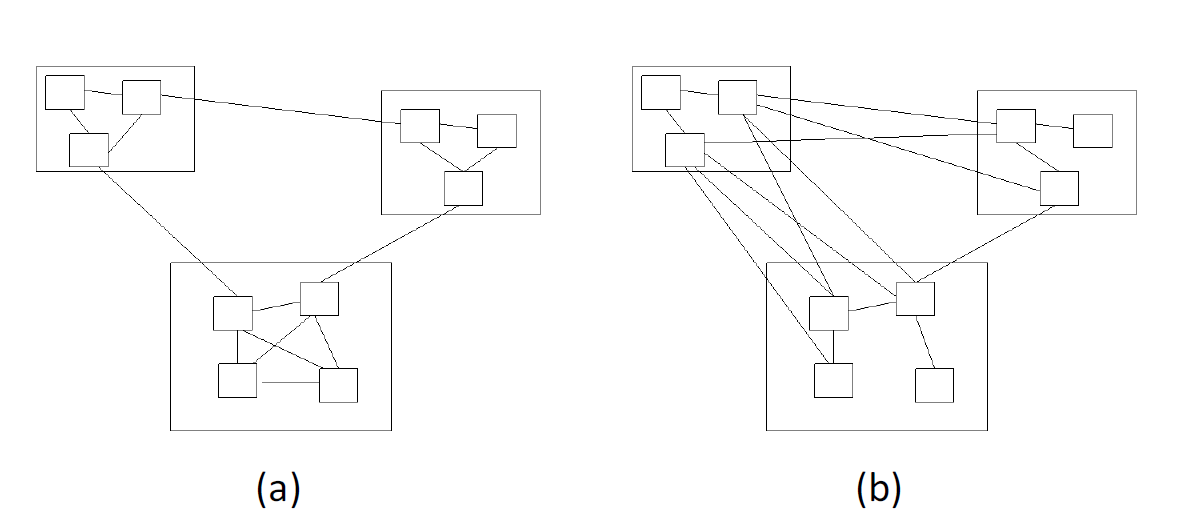
\includegraphics[width=\linewidth]{images/Modularisierung/BeispieleKopplungKohaesion.png}
\vfill\null
\begin{itemize}
	\item Bild a: Schwache Kopplung, starke Kohäsion (gut)
	\item Bild b: Starke Kopplung, schwache Kohäsion (schlecht)
\end{itemize}
\vfill\null
\end{multicols}

\begin{multicols}{2}
\subsection{Definitionen Kopplung}
\begin{itemize}
  \item Keine direkte Kopplung (Schwache Kopplung $\rightarrow$ \textbf{GUT})
  \item Datenkopplung
  \begin{itemize}
    \item Kommunikation ausschliesslich über Parameter
  \end{itemize}
  \item Datenbereichskopplung
   \begin{itemize}
    \item Modul hat Zugriff auf Datenstruktur eines anderen Moduls
    \item Es werden nur einzelne Komponenten benötigt
  \end{itemize}
  \item Steuerflusskopplung (Control Flow)
  \begin{itemize}
    \item Modul beeinflusst Steuerfluss eines anderen Moduls
  \end{itemize}
  \item Globale Kopplung
  \begin{itemize}
    \item Kommunikation über globale Variabeln
    \item Jedes Modul hat Zugriff
  \end{itemize}
  \item Inhaltskopplung (Starke Kopplung $\rightarrow$ \textbf{SCHLECHT})
  \begin{itemize}
    \item Aus einem Modul werden lokale Daten eines anderen Moduls modifiziert,
    obwohl dieses Modul NICHT vom anderen Modul aufgerufen wird.
    \item \textbf{Todsünde}
  \end{itemize}
\end{itemize}
\columnbreak
\subsection{Definitionen Kohäsion}
\begin{itemize}
  \item Funktionale Kohäsion (Starke Kohäsion $\rightarrow$ \textbf{GUT})
  \begin{itemize}
    \item Teile einer Einheit bilden zusammen eine Funktion
  \end{itemize}
  \item Sequentielle Kohäsion
   \begin{itemize}
    \item Teilfunktionen einer Einheit werden nacheinander ausgeführt
    \item Das Ergebnis einer Teilfunktion ist die Eingabe der nächsten
  \end{itemize}
  \item Kommunikative Kohäsion
  \begin{itemize}
    \item Teilfunktionen einer Einheit werden auf den gleichen Daten ausgeführt
    \item Reihenfolge spielt keine Rolle
  \end{itemize}
  \item Prozedurale Kohäsion
  \begin{itemize}
    \item Teilfunktionen werden nacheinander ausgeführt
    \item Sind über Steuerfluss verknüpft
  \end{itemize}
  \item Zeitliche Kohäsion
  \begin{itemize}
    \item Teile einer Einheit sind alle zu einer bestimmten Zeit auszuführen
  \end{itemize}
  \item Logische Kohäsion
  \begin{itemize}
    \item Teilfunktionen einer Einheit gehören zu einer Klasse
  \end{itemize}
  \item Zufällige Kohäsion (Schwache Kohäsion $\rightarrow$ \textbf{SCHLECHT})
  \begin{itemize}
    \item Teilfunktionen einer Einheit haben keinen sinnvollen Zusammenhang
  \end{itemize}
\end{itemize}
\end{multicols}
\begin{minipage}{9cm}
\subsubsection{Ziele bezüglich Kohäsion}
  \begin{itemize}
  \item Kohäsion maximieren
  \item Idealerweise führt eine Unit nur eine Aufgabe (Funktion) aus
  \item Starke Kohäsion steigert
    \begin{itemize}
    \item Wartbarkeit
    \item Änderbarkeit
    \item Verständlichkeit
    \end{itemize}
  \item \textbf{Zusammengehörendes zusammen nehmen!}
  \item \textbf{Starke Kohäsion führt zu schwacher Kopplung, aber nicht umgekehrt!!}
  \end{itemize}
\end{minipage}
\hfill
\begin{minipage}{9cm}
  \subsubsection{Bestimmung der Kohäsion}
  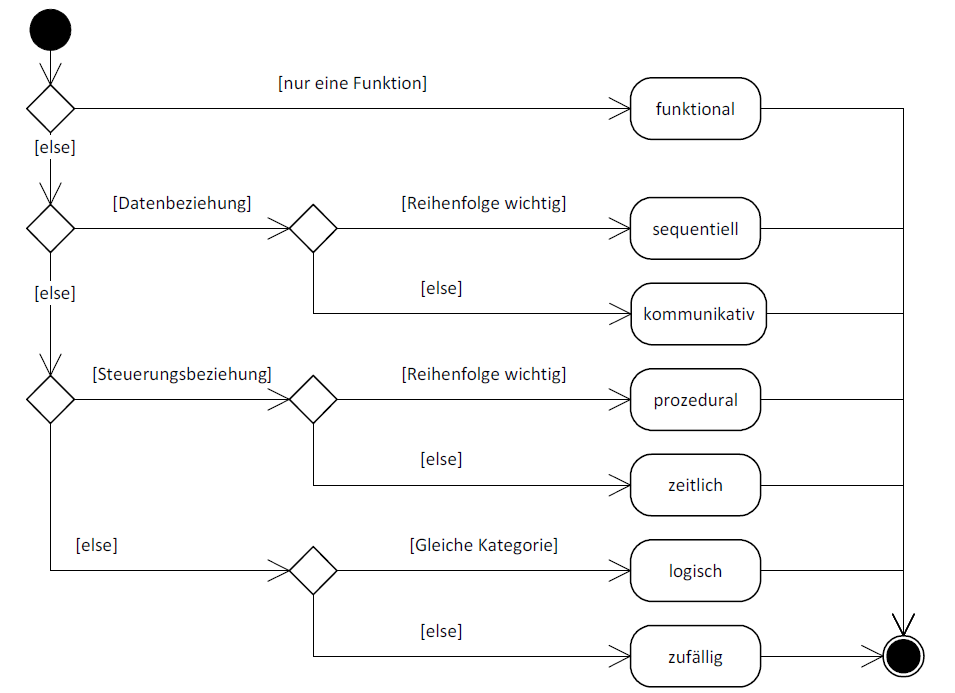
\includegraphics[width=9cm]{images/Modularisierung/Kohaesionsbestimmung.png}
\end{minipage}

\subsection{Schlechte vs. gute Modularisierung}
\begin{minipage}[t]{10cm}
\textbf{Beispiel schlechter Modularisierung:}\\
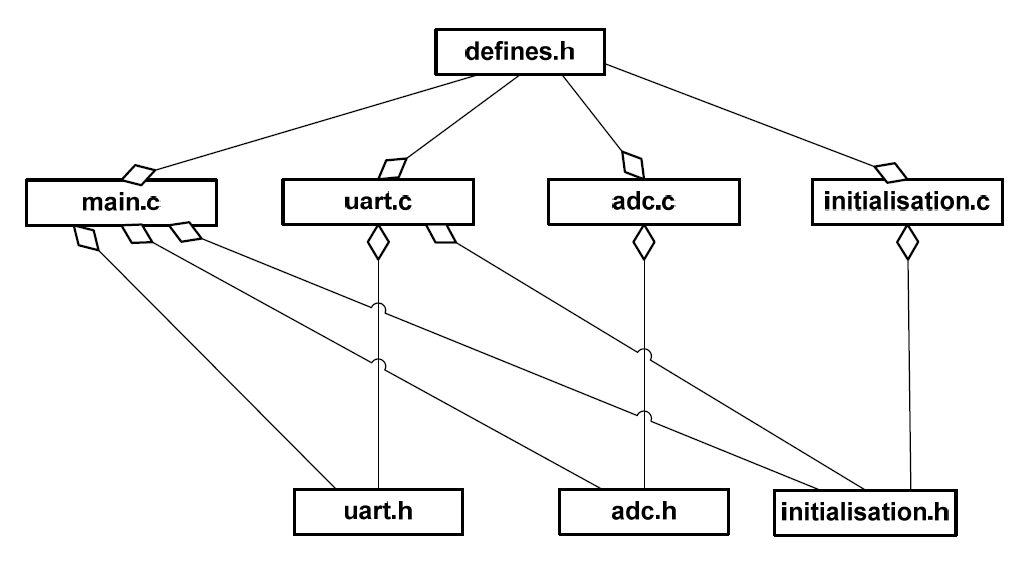
\includegraphics[width=9cm]{images/Modularisierung/SchlechtesBeispielModularisierung.png}
\end{minipage}
\begin{minipage}[t]{8cm}
\textbf{Beispiel guter Modularisierung:}\\
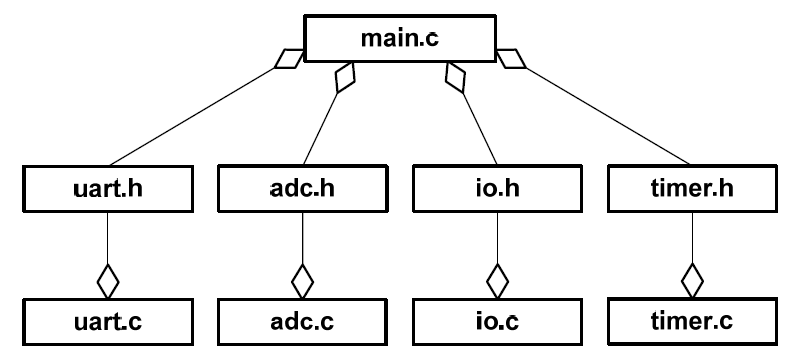
\includegraphics[width=8cm]{images/Modularisierung/GutesBeispielModularisierung.png}
\end{minipage}

\subsection{In bestehendem Projekt zurechtfinden}
\begin{itemize}
	\item Die Schnittstelle muss in den Headerfiles beschrieben werden
	\item Dort muss man alles finden, was wichtig ist, d.h. es müssen zuerst die Headerfiles studiert werden
	\item Wenn man das Projekt nur nutzen soll, dann sollte man im Normalfall keinen Grund finden, auch die Definitionsfiles (*.c, *.cpp) anschauen zu müssen
\end{itemize}

\subsection{Package-Diagramm}
\begin{itemize}
	\item ist bekannt aus OOAD
	\item Ein Package besteht aus mindestens einer, üblicherweise aus mehreren Klassen, die zusammengehören (Stichwort: Kohäsion)
	\item Im Package-Diagramm kann dargestellt werden, welche Packages mit welchen anderen Packages Verbindungen haben (dürfen), d.h. die Abhängigkeiten zwischen Packages können sichtbar gemacht werden
	\item In C++ wird das Packagekonzept mit Namespaces umgesetzt, d.h. ein Namespace entspricht einem Package
\end{itemize}
